\documentclass[conference]{IEEEtran}
% \IEEEoverridecommandlockouts
% The preceding line is only needed to identify funding in the first footnote. If that is unneeded, please comment it out.
\usepackage{cite}
\usepackage{amsmath,amssymb,amsfonts}
\usepackage{algorithmic}
\usepackage{graphicx}
\graphicspath{ {./img/} }
\usepackage{csvsimple}
\usepackage{textcomp}
\usepackage{xcolor}
\usepackage{tikz}
\def\BibTeX{{\rm B\kern-.05em{\sc i\kern-.025em b}\kern-.08em
    T\kern-.1667em\lower.7ex\hbox{E}\kern-.125emX}}
\begin{document}

%%%%%%%%%%%%%%%%%%%%%%%%%%%%%%%%%%%%%%%
% TITLE
%%%%%%%%%%%%%%%%%%%%%%%%%%%%%%%%%%%%%%%
\title{SimHome: Predicting Potentially Wasteful Energy Consumption}

%%%%%%%%%%%%%%%%%%%%%%%%%%%%%%%%%%%%%%%
% Authors
%%%%%%%%%%%%%%%%%%%%%%%%%%%%%%%%%%%%%%%

% COLUMN 1
\author{
\IEEEauthorblockN{Arthur Liu}
\IEEEauthorblockA{\textit{University of California, Irvine} \\
\textit{Computer Science and Engineering}
} \\
\IEEEauthorblockN{Prof. G.P. Li}
\IEEEauthorblockA{\textit{University of California, Irvine} \\
\textit{Advisor - CalPlug Research Laboratory}
}

% COLUMN 2
\and
\IEEEauthorblockN{Brian Tom}
\IEEEauthorblockA{\textit{University of California, Irvine} \\
\textit{Computer Science and Engineering}
} \\ % ADD IT FOR SAME COLUMN
\IEEEauthorblockN{Dr. Michael Klopfer}
\IEEEauthorblockA{\textit{University of California, Irvine} \\
\textit{Advisor - CalPlug Research Laboratory}
}

% COLUMN 3
\and
\IEEEauthorblockN{Fernan Lukban}
\IEEEauthorblockA{\textit{University of California, Irvine} \\
\textit{Computer Science and Engineering}
}
}
\maketitle


%%%%%%%%%%%%%%%%%%%%%%%%%%%%%%%%%%%%%%%
% ABSTRACT
%%%%%%%%%%%%%%%%%%%%%%%%%%%%%%%%%%%%%%%
\begin{abstract}
Our goal is to save energy by automatically notifying users of wasteful energy usage. With energy usage is at an all-time high, combined with rising energy rates, wasteful energy usage is not only bad from an environmental standpoint but an economic standpoint. Instead of trying to create a new, more efficient means of energy production, we instead try to minimize potential misuse of devices to save energy and money by applying modern machine learning techniques. Long Short-Term Memory recurrent neural networks allow us to analyze energy consumption trends with respect to both long- and short-term trends. Our model, stored in Google Cloud's AI Platform, receives data from our MySQL database via an API to generate predictions about future energy consumption. Through our Slack interface, we can query predicted energy consumption specific SimHome devices for the next minute or hour.
\end{abstract}

% Probably not needed
% \begin{IEEEkeywords}
% component, formatting, style, styling, insert
% \end{IEEEkeywords}


%%%%%%%%%%%%%%%%%%%%%%%%%%%%%%%%%%%%%%%
% INTRODUCTION
%%%%%%%%%%%%%%%%%%%%%%%%%%%%%%%%%%%%%%%
\section{Introduction}
Growing energy demands throughout the world due to increased dependence on electronic devices, especially throughout California, have put increasing pressure on utility company infrastructures. Combined with the recent wildfires sparked by faulty utility equipment, we wanted to provide methods of reducing energy consumption. Specifically, our goal was to reduce wasteful energy consumption on plug loads using predictive models and provide an actionable user interface to better manage their energy consumption. A study by Klopfer on energy consumption in the classroom utilized predictive models on projector energy consumption, finding a correlation between energy usage and environmental conditions (light, movement, etc.) \cite{b3}. Our solution provides automated energy management by analyzing behavior patterns with environmental sensors and is an improvement to the manual energy-saving methods suggested by Pigg \cite{b2}.

\section{Materials and Testing Environment}
\subsection{Materials}
\begin{itemize}
    \item IoT energy, movement, and temperature sensors
    \item Wi-Fi Network and cloud compute service
    \item Server for hosting website
    \item Multi-state power appliances
\end{itemize}

\subsection{SimHome Environment}
The SimHome (Simulation Home) is our test environment for collecting energy usage, temperature, and motion data. Throughout the home, we have various appliances, such as a refrigerator, microwave, television, and lamp connected to smart plugs that monitor energy usage throughout the SimHome. The smart plugs are supplied by Smartenit, a local Internet of Things (IoT) company that we work with. The plugs report instantaneous demand in watts, on/off data, and cumulative energy totals. We also utilize Onset HOBO Data Loggers that provide power, motion, and light readings for more focused studies throughout the office.

\section{Long Short-Term Neural Networks}
To generate predictions about potentially wasteful energy usage, we built a Long-Short Term Memory (LSTM) Recurrent Neural Network (RNN). LSTM neural networks, as the name implies, utilize a combination of long-term persistent “memories” and short-term observations to predict future values. Unlike alternative recurrent neural networks that make predictions based on a fixed historical window, LSTMs can remember long-term dependencies.

A previous study performed by Klopfer et. al used Linear Support Vector Machine (SVM) to model video projector energy consumption but only trained under optimum training conditions and about 3.67 minutes of data \cite{b3}. They also noted that Linear SVM may cause inappropriate shutdowns as learning certain patterns were more difficult. LSTMs were suggested to help learn more complex user patterns for making better energy saving suggestions.

Our LSTM neural network currently uses a single hidden LSTM layer (making local training easier) with a dense output layer, as shown in Figure \ref{fig:lstm_model}. We kept the model simple for now to test out the feasibility of LSTMs on our data before training the model in the Google Cloud Platform.

\begin{figure}[htbp]
    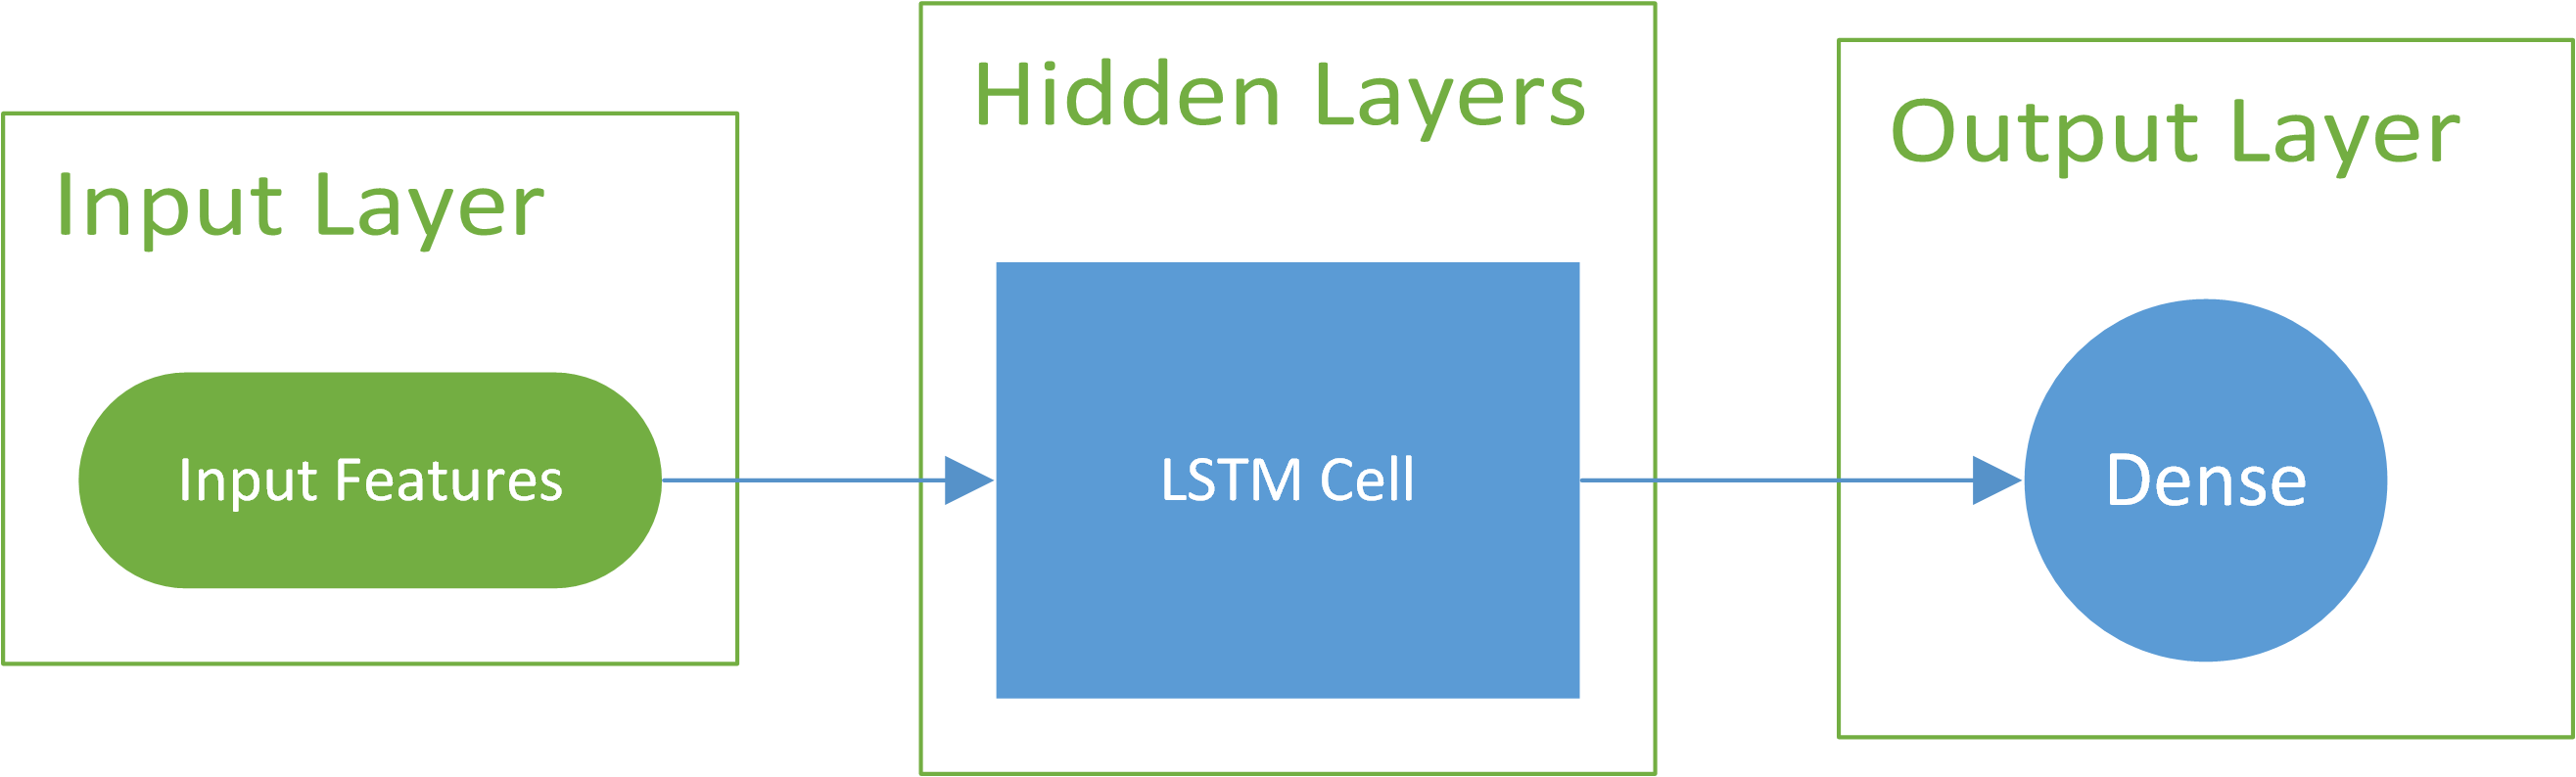
\includegraphics[width=\linewidth]{img/model.png}
    \caption{Simple LSTM neural network containing a single hidden layer.}
    \label{fig:lstm_model}
\end{figure}

\section{Data Collection}
The data collection system consists of a Python package deployed to our central data aggregation system managed by Smartenit. Our software processes data received over MQ Telemetry Transport (MQTT), a pub-sub messaging protocol, that allows us to filter messages from the Smartenit smart plugs based on our selected subscriptions. The MQTT protocol will asynchronously send messages to our script, which pushes the data to a MySQL database.  Additionally, we have data from HOBO sensors that monitor computer usage, light, and occupancy. A sample of the data is shown in Figure \ref{fig:data_hobo}.

\begin{figure}[h]
	\centering
	\csvautotabular[filter={\value{csvrow}<10}]{data/data_hobo.csv}
	\caption{A few columns of training data from a HOBO data logger attached to an office PC. Records are logged every 10 seconds. Our goal is to predict the \texttt{Energy} column.}
	\label{fig:data_hobo}
\end{figure}

\section{Learning and Prediction Platform}
This platform encompasses the union between the Data Collection System as well as our LSTM RNN. The learning and prediction platform is tasked with learning using the data collection system and creating notifications to send to the notification platform.

\subsection{Constraints}
\begin{itemize}
    \item Easy to scale along with the growing data set
    \item Able to concurrently improve and apply predictions
    \item Able to incrementally learn from the ever-growing data set
\end{itemize}

\subsection{Solution}
Since both our LSTM RNN and our data collection system is implemented in Python, we also decided to implement our learning and prediction platform in Python as well. Our model loss was very good as shown in Figure \ref{fig:model_loss}, though we need to test our model on out of sample data to verify whether it generalizes well \cite{b4}. Sample predictions from our LSTM model developed in TensorFlow are shown in Figure \ref{fig:prediction02}. As for the software design, we decided to separate the incremental learning and the prediction construction into two separate Python processes. This allows us to easily scale horizontally with great flexibility. If we need faster incremental learning, then we can just spawn more incremental learning subsystems and vice versa. We designed this system as a pipeline that takes data from the data collection system, processes it in the incremental learning subsystem, which then updates the weights and predictions, where the results get sent to the prediction construction subsystem. Finally, the prediction construction subsystem then creates notifications where the notification system will use the information to notify users of wasteful energy usage.

\begin{figure}[htbp]
    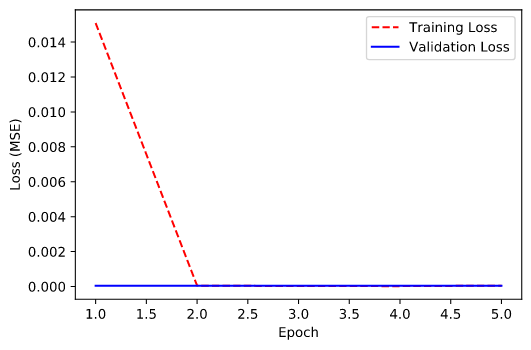
\includegraphics[width=\linewidth]{img/loss.png}
    \caption{The mean-square error (MSE) loss on training and validation data. Our training data contained about 230,000 rows and we used a 70/30 training-validation split to develop our model. The error is close the zero, but we need to perform cross-validation and testing with additional data to verify our model.}
    \label{fig:model_loss}
\end{figure}

\begin{figure}[htbp]
    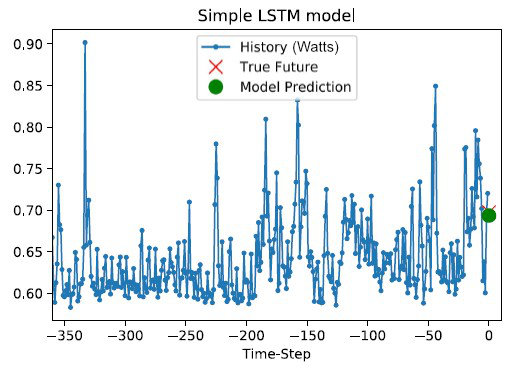
\includegraphics[width=\linewidth]{img/prediction02.jpg}
    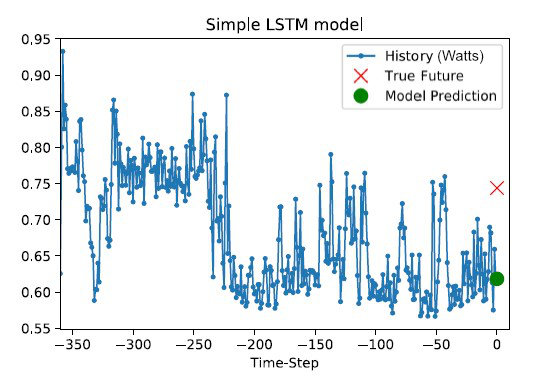
\includegraphics[width=\linewidth]{img/prediction03.jpg}
    \caption{These graphs show that our model cannot handle all patterns yet. The predictions, however, were very close to the expected results. We will need to refine our model and gather more data to make better predictions.}
    \label{fig:prediction02}
\end{figure}

\subsection{Implementation}
These subsystems which make up our learning and prediction platform are implemented using MQTT, the messaging pub-sub system that our data collection system utilizes. This provided us great speed in developing as we could reuse a lot of our existing code. The pipeline between the systems is implemented as a message processor that processes each message based on the payload and then forwards the result to the next step in the pipeline. The incremental learning subsystem receives the data in the form of subscription messages from our data collection system, learns from the data, and then forwards the results to our prediction construction subsystem. This prediction construction subsystem then examines the changes, where it will choose to either update the weights of its model or create a notification. The notification created can then be consumed by the notification platform.

\subsection{Functionality}
\begin{itemize}
    \item Can bring up new servers to scale horizontally
    \item Uses data pipeline to incrementally improve updates
    \item Constructs predictions and notifications in real-time using data
\end{itemize}

\section{Notification Platform}\label{Notification Platform}
The notification platform is a long-lived process that interacts directly with users about their wasteful energy usage. Most of the interactions will be driven from the server-side, with some input from the users.

\subsection{Constraints}
\begin{itemize}
    \item Establish a connection between a user and the server
    \item Keep that connection open so that we can send notifications
    \item Drive notifications using predictions from the prediction platform
    \item Allow us to turn on and off devices remotely using the sensor API
    \item Secure from any eavesdropping between server and client
\end{itemize}

\subsection{Solution}
After evaluating the pros and cons of our possible solutions, we decided to go with WebSockets since the REST API would not be able to keep the connection open \cite{b5}. WebSockets are also more robust and allow us to reuse our notification platform for different user interfaces \cite{b6}.

\subsection{Implementation}
The notification platform is implemented in Python using the open-source WebSockets library. This library was much better compared to the other web socket library since it had support for the new asyncio library in Python. This means that it had native language async support, allowing our code to be fast and maintainable for the foreseeable future. The WebSockets library which uses TCP is a lot harder to spoof and has built-in packet re-transmission and reordering.

\subsection{Functionality}
\begin{itemize}
    \item Allow a user to login
    \item Receive notifications
    \item List devices
    \item Send requests to turn off devices
\end{itemize}

\section{Slack Bot}
After setting up all the hardware and the backend system, we implemented the frontend to make our system more user-friendly. Although web applications and smart home devices can display energy usage data, we want the system to take actions for users through the frontend. To achieve those goals, we built an automatic chatbot on Slack to enable user interaction.

A Slack bot is a type of Slack App designed to interact with users via direct conversation. With the support of the backend database and the API protocol, Slack bot can communicate with users without the need to manually taking actions from our end.

\subsection{Implementation}
The Slack bot uses Dialogflow as a natural language process platform. Dialogflow parses the user input and recognizes essential tokens to retrieve data from the backend accordingly. It will prune all other invalid user inputs to keep the Slack bot system stable and consistent.

When the user logs in the Slack, the user’s unique account information will be linked to our backend and retrieve the unique prediction model. The slack bot will bind the authentication and make the proper API call to ensure data will be sent to the right user.

The Slack bot can receive input and react base on it, as shown in Figure \ref{fig:slack}. The inputs come from two resources including user end and system end. The user end can send a request to ask about the energy usage and take actions (turn on/off the devices). Besides, users can view the device lists and modify it through Slack bot. The system end will detect the wasteful energy usage through the LSTM neural network and send a notification through Slack bot to nudge users to take action. Users can choose either to turn off the devices that might overuse the energy or to leave them on depends on their personal preference.

\begin{figure}[htbp]
    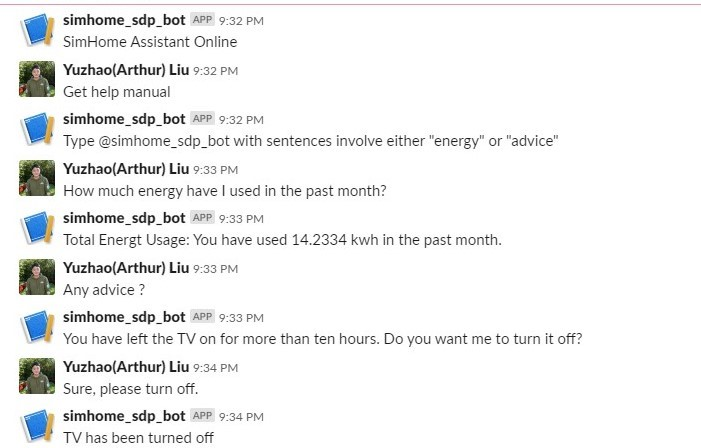
\includegraphics[width=\linewidth]{img/slack.jpg}
    \caption{Demonstrating a conversation between Slack and a user.}
    \label{fig:slack}
\end{figure}

The users’ activities through the Slack bot will be recorded and send back to the backend through the Slack bot. The LSTM neural network will use those records to retrain the model and improve the prediction. If our model recognizes the wasteful energy usage but does not receive any response from the Slack bot, the system will turn off the electronic device base on the prediction and send a Slack notification back to users. By doing so, the users know what happened to the electronic devices, which enables them to give feedback.

\section*{Summary}
We developed our automatic system by creating two platforms: one for processing data as well as creating predictions and one for driving the user interactions. To process the data we used the already existing SimHome webserver to collect data and send it to the data platform that we created. This data collection system feeds into our learning and prediction platform, which incrementally improves our models and creates predictions. We implemented this as a WebSocket which any language or implementation can access due to ease of maintainability and development time. This platform was then hosted in the cloud using the Google Cloud Platform. This is done so that the learning and prediction can be done significantly faster as opposed to using local servers. Once these predictions are created, they can then be accessed by the notification system which drives user interaction. To query the learning and prediction platform, API calls can be made to the Google Cloud Platform with the payload including time slices of the data. It is through this API that the granularity of the calls can be changed, allowing predictions on different timescales. The user interface we created was a Slack bot which allows us to directly talk to users about their energy usage.

\section*{Conclusion}
While we accomplished a lot with our project this quarter, there are still many things to improve. We intend to expand our project by improving the bottlenecks in our system. Last quarter, we identified our bottleneck as the neural network and moved it to the cloud to improve our learning and prediction platform. We found that despite the time it took to re-implement our prediction platform, we were able to access this system anywhere while allowing us to gather more data for training and testing. In addition, we improved the granularity of our energy prediction period. Now, the next logical step is to provide new ways to interact with our system by building either a web app or a phone app. 

The most important part that we want to include, is a new way to interact with our system. The most important distinction between our research and the work of others before us is our dedication to user interaction [1-3]. We believe that though the science is important, it is not useful unless it can be applied to a real-world problem. To solve this, we plan to either create a web app or phone app which will be the main avenue that our users will receive their notifications. The first thing we want to do is move towards a native app, on either iOS or Android. This will overall allow users to reflect on their data trends. Having a main gathering place to see data on a phone will be paramount as many people now rely on their phones for information.

\section*{Acknowledgment}
Thanks to everyone on the SimHome team including Arthur Liu, Brian Tom, and Fernan Lukban for all your efforts on this project. Special thanks to our advisors Dr. Michael Klopfer and Prof. G.P. Li. for providing us with guidance throughout our development process. We would not have been able to make so much progress in such little time without your support.

Additionally, thanks to the Undergraduate Research Opportunities Program (UROP) for providing funding for our SimHome environment and various cloud tools we have used to train our models more quickly.

Finally, thanks to Al Choperena and Dhawal Doshi at Smartenit for supplying CalPlug with smart sensors and providing our team with troubleshooting advice whenever needed.

\begin{thebibliography}{00}
\bibitem{b1} M. Fayaz and D. Kim, ``A Prediction Methodology of Energy Consumption Based on Deep Extreme Learning Machine and Comparative Analysis in Residential Buildings,`` Electronics, vol. 7, no. 10, p. 222, 2018.
\bibitem{b2} S. Pigg, I. Bensch, and K. Koski, ``Energy Savings Opportunities with Home Electronics and Other Plug-Load Devices: Results from a Minnesota Field Study,`` ACEEE Summer Study on Energy Efficiency in Buildings. Pacific Grove (Calif.): American Council for An Energy Efficient Economy (Washington, DC), 2010.
\bibitem{b3} M. Klopfer, Z. Chen, U. Kazmi, S. Kasat, and J. Pixley, ``Energy management in projectors and display technology by use of predictive behavior models,`` California Plug Load Research Center (CalPlug), University of California, Irvine, 2018.
\bibitem{b4} C. Olah, ``Understanding LSTM Networks.`` Aug. 27, 2015. [Online]. Available: https://colah.github.io/posts/2015-08-Understanding-LSTMs
\bibitem{b5} Sye Loong Keoh, Sandeep S. Kumar, Hannes Tschofenig, ``Securing the Internet of
Things: A Standardization Perspective``, Internet of Things Journal IEEE (Volume:
1, Issue: 3), pp. 265-275, June 2014.
\bibitem{b6} P. Lubbers and F. Greco, ``HTML5 Web Sockets: A Quantum Leap in Scalability for the Web,`` SOA World Magazine, Mar. 2010; http://soa.sys-con.com/node/1315473.
\end{thebibliography}

% Removed Appendix

\end{document}